\chapter{Принцип максимума для уравнения теплопроводности в ограниченной области. Единственность решения первой краевой задачи.}
\label{cha:10}

Пусть $x \in \mathbb{R}^n \text{ -- координата, } t \in \mathbb{R} \text{ -- время.}, \; u(t, \bar{x})$ -- температура стержня в точке x в момент времени t. Тогда \red{уравнение теплопроводности} записывается следующим образом:
$$u_t = a^2 \Delta_x u \equiv a^2(u_{x_1x_1} + \ldots + u_{x_nx_n})$$

\begin{theorem}[\red{принцип максимума в ограниченной области (в стакане)}]
	Пусть задано уравнение теплопроводности $u_t = a^2 \Delta_x u$ в некоторой области $\Omega = \lbrace 0 < x < l, \; 0 < t < T \rbrace$. 

	\begin{multicols}{2}
		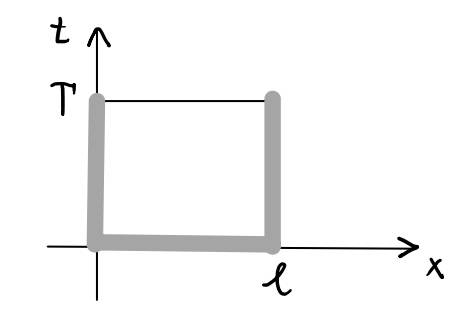
\includegraphics[scale=0.3]{cha10im3} 

		\columnbreak

		Имеем границу: 

		$\Sigma = \lbrace x = 0 \rbrace \cup \lbrace x = l \rbrace \cup \lbrace t = 0 \rbrace$\\

		Также пусть заданы величины: 

		$m = \underset{\Sigma}{min}(u)$ и $M = \underset{\Sigma}{max}(u)$
	\end{multicols}
	
	Тогда:
	$$m \le u(t, \overline{x}) \le M \; \forall (t, \overline{x}) \in \Omega $$
\end{theorem}
\begin{Proof}
	\blue{(от противного)}

	Докажем для утверждение для максимума, для минимума доказательство аналогично. 

	Пусть $max$ достигается в точке $ (t_0, x_0) $ внутри $\Omega$ или на $ t = T $. Введем вспомогательную функцию:
	$$\begin{gathered}
		u_\varepsilon(t, x) = u(t, x) + \varepsilon x^2 \\
		\text{(для }min: \;  u_\varepsilon(t, x) = u(t, x) - \varepsilon x^2\text{)}
	\end{gathered}$$
	Пусть $max \; u_\varepsilon(t, x) $ - точка $ (t_1, x_1) $ внутри $\Omega$ или на $t = T$, т.е.:\\

	\begin{figure}[h]
		\begin{multicols}{2}
			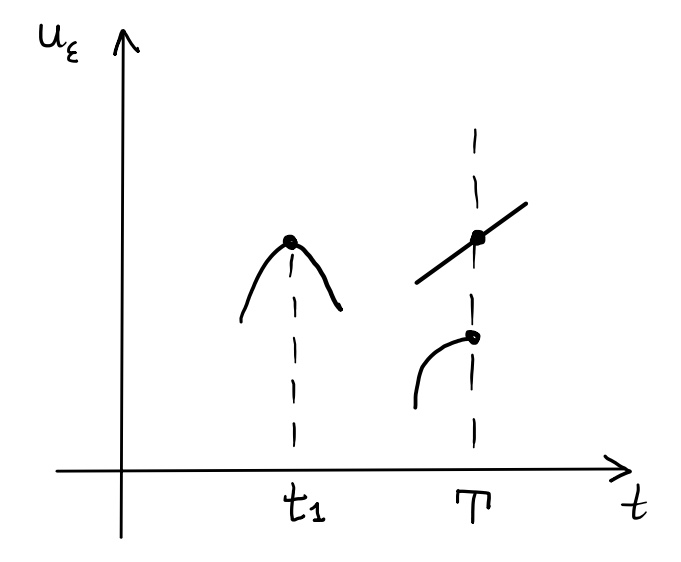
\includegraphics[width=70mm]{cha10im1}

			\begin{center}
				$\begin{cases}
					\text{либо } (u_\varepsilon)_t(t_1, x_1) = 0, \; t_1 < T \\
					\text{либо } (u_\varepsilon)_t(t_1, x_1) < 0, \; t_1 = T \\
					\text{либо } (u_\varepsilon)_t(t_1, x_1) = 0, \; t_1 = T
				\end{cases}$
			\end{center}

			\columnbreak
			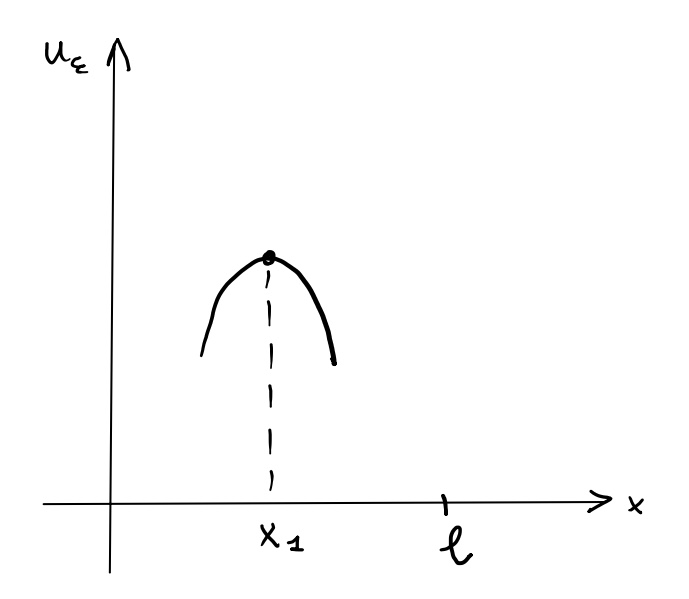
\includegraphics[width=70mm]{cha10im2}
			
			$\;\;\;\;\;\;\;\;\;\;\;\;(u_\varepsilon)_{xx}(t_1, x_1) \le 0$
		\end{multicols}
	\end{figure}

	% \begin{figure}[h]
	% 	\begin{center}
	% 		\begin{minipage}[h]{0.45\linewidth}
	% 		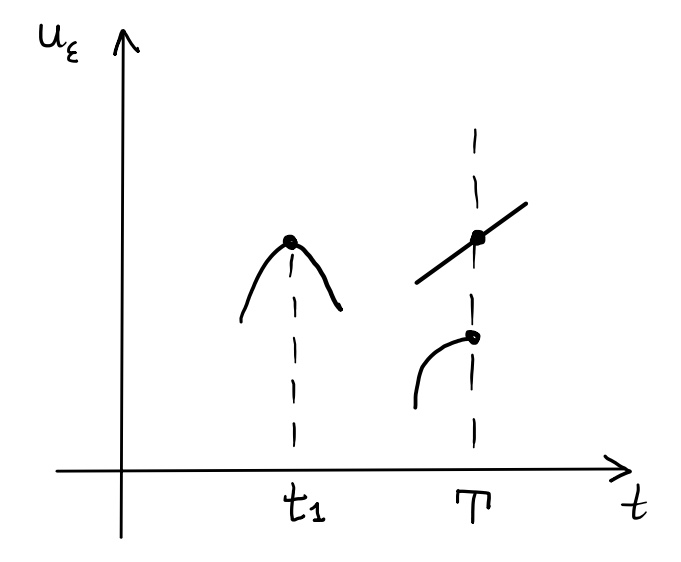
\includegraphics[width=1\linewidth]{cha10im1}
	% 		\end{minipage}
	% 		\begin{minipage}[h]{0.45\linewidth}
	% 		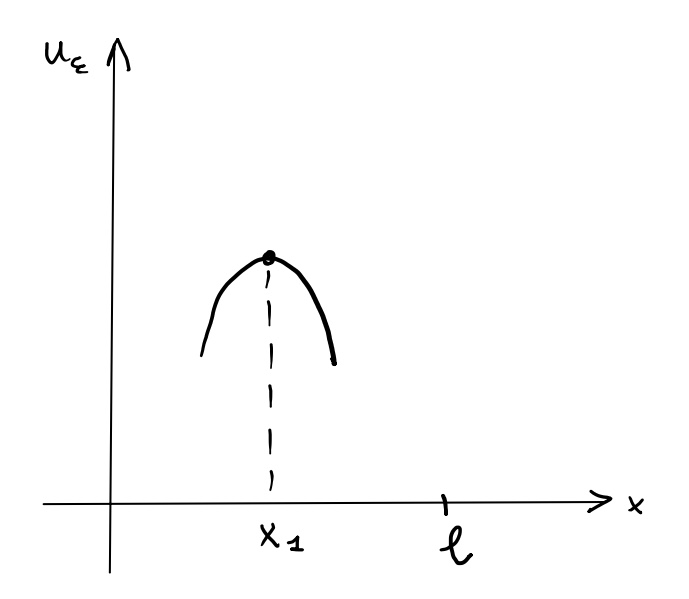
\includegraphics[width=1\linewidth]{cha10im2}
	% 		\end{minipage}
	% 	\end{center}
	% \end{figure}

	$$\begin{gathered}
		\underbrace{(u_\varepsilon)_t}_{\ge 0} - \underbrace{a^2(u_\varepsilon)_{xx}}_{\le 0} \ge 0$ в $ (t_1, x_1) \\
		(u_\varepsilon)_t - a^2(u_\varepsilon)_{xx} = \underbrace{u_t - a^2u_{xx} }_{= 0}- 2\varepsilon a^2 = -2a^2\varepsilon < 0
	\end{gathered}$$
	Получаем противоречие, значит $max \in \Sigma $.
	
\end{Proof}

\begin{conseq}[\red{единственность решения 1-ой краевой задачи}]
	Пусть имеем 1-ую краевую задачу:
	$$\begin{cases}
		u_{t} = a^2 u_{xx}, \; t > 0, \; x \in (0, l)\\
		u|_{t = 0} = \varphi (x) \\
		u|_{x = 0} = \mu (t) \\
		u|_{x = l} = \nu (t)
	\end{cases}$$
	Тогда ее решение существует и единственно.
\end{conseq}
\begin{Proof}
Предположим, что $ \exists \; u_1, \; u_2 $ -- решения такие, что $ u_1 \neq u_2.$ Введем $z = u_1 - u_2 $, тогда для $z$ имеем следующую задачу:
$$\begin{cases}
	z_{t} = a^2 z_{xx}, \; t > 0, \; x \in (0, l)\\
	z|_{t = 0} = 0 \\
	z|_{x = 0} = 0 \\
	z|_{x = l} = 0
\end{cases}$$.
Используя принцип максимума, получаем, что $ z \equiv 0 \Longrightarrow u_1 = u_2 $.
\end{Proof}

